%--- Title Page -------------------------------------------------------%
\maketitle

%--- Table of Contents-------------------------------------------------%
% For longer table of contents, I find it cleaner to
% use no footline.
\setcounter{tocdepth}{1}
\begin{frame}[plain, noframenumbering]{Outline}
	\begin{multicols}{2}
		\tableofcontents
	\end{multicols}
\end{frame}

%--- Distributions ----------------------------------------------------%

\tikzset{
	declare function={
			discreteuniform(\a,\b)=1/(\b-\a+1);%
			binomial(\n,\p)=\n!/(x!*(\n-x)!)*\p^x*(1-\p)^(\n-x);%
			poisson(\l)=(\l^x)*exp(-\l)/(x!);%
			negativebinomial(\r,\p)=((x+\r-1)!/((\r-1)!*x!))*((1-\p)^x*\p^\r);%
			continuousuniform(\a,\b)=1/(\b-\a);%
			gaussian(\m,\s)=1/(\s*sqrt(2*pi))*exp(-((x-\m)^2)/(2*\s^2));%
			lognormal(\m,\s)=1/(x*\s*sqrt(2*pi))*exp(-((ln(x)-\m)^2)/(2*\s^2));%
			exponential(\l)=\l*exp(-\l*x);%
			gamma(\z)=2.506628274631*sqrt(1/\z)+ 0.20888568*(1/\z)^(1.5)+ 0.00870357*(1/\z)^(2.5)- (174.2106599*(1/\z)^(3.5))/25920- (715.6423511*(1/\z)^(4.5))/1244160)*exp((-ln(1/\z)-1)*\z;%
			gammadist(\a,\t)=(x^(\a-1))*exp(-x/\t)*gamma(\a)*\t^\a;%
			student(\n)=gamma((\n+1)/2.)/(sqrt(\n*pi)*gamma(\n/2.))*((1+(x*x)/\n)^(-(\n+1)/2.));%
			cauchy(\m,\s)=(1/(pi*\s*(1+((x-\m)/\s)^2)));%
			beta(\a,\b)=(x^(\a-1)*(1-x)^(\b-1)/((gamma(\a)*gamma(\b))/gamma(\a+\b));%
			binormal(\ma,\sa,\mb,\sb,\ro)=exp(-(((x-\ma)/\sa)^2+((y-\mb)/\sb)^2-(2*\ro)*((x-\ma)/\sa)*((y-\mb)/\sb))/(2*(1-\ro^2)))/(2*pi*\sa*\sb*(1-\ro^2)^0.5);%
			conditionalbinormal(\yc,\ma,\sa,\mb,\sb,\ro)=exp(-(((x-\ma)/\sa)^2+((\yc-\mb)/\sb)^2-(2*\ro)*((x-\ma)/\sa)*((\yc-\mb)/\sb))/(2*(1-\ro^2)))/(2*pi*\sa*\sb*(1-\ro^2)^0.5);%
			sumtwonormals(\ma,\sa,\wa,\mb,\sb,\wb)=(\wa*gaussian(\ma,\sa))+(\wb*gaussian(\mb,\sb));%
			normcdf(\m,\s)=1/(1 + exp(-0.07056*((x-\m)/\s)^3 - 1.5976*(x-\m)/\s));%
		}
}

%--- Files ----------------------------------------------------------%
% !TeX root = slides.tex

\section{Pumas}
\begin{frame}{What is Pumas?}
    Pumas (\textbf{P}harmace\textbf{U}tical \textbf{M}odeling \textbf{A}nd \textbf{S}imulation)
    \parencite{rackauckas2020accelerated}
    is a suite of tools to perform quantitative analytics of various kinds
    across the horizontal of pharmaceutical drug development.
    The purpose of this framework is to bring efficient implementations of
    all aspects of the analytics in this domain under one cohesive package.
\end{frame}

\begin{frame}{Pumas Features}
    Pumas 2.3 currently includes:
    \begin{vfilleditems}
        \small
        \item Non-compartmental Analysis
        \item Specification of Nonlinear Mixed Effects (NLME) Models
        \item Simulation of NLME model using differential equations or analytical solutions
        \item Deep control over the differential equation solvers for high efficiency
        \item Estimation of NLME parameters via Maximum Likelihood, Expectation Maximization and Bayesian methods
        \item Parallelization capabilities for both simulation and estimation
        \item Mixed analytical and numerical problems
        \item Simulation and estimation diagnostics for model post-processing
        \item Interactive model exploration and diagnostics tools through webapps
        \item Automated report generation for models and non-compartmental analysis
        \item Global and local sensitivity analysis routines for multi-scale models
        \item Bioequivalence analysis
        \item Optimal design of experiments
    \end{vfilleditems}
\end{frame}
\include{01-Bayesian_Statistics}
\section{Priors}

\subsection{Recommended References}
\begin{frame}{Priors and Posteriors - Recommended References}
	\begin{vfilleditems}
		\item \textcite{gelman2013bayesian}:
		\begin{vfilleditems}
			\item Chapter 2: Single-parameter models
			\item Chapter 3: Introduction to multiparameter models
		\end{vfilleditems}
		\item \textcite{mcelreath2020statistical} - Chapter 4: Geocentric Models
		\item \textcite{gelman2020regression}:
		\begin{vfilleditems}
			\item Chapter 9, Section 9.3: Prior information and Bayesian synthesis
			\item Chapter 9, Section 9.5: Uniform, weakly informative, and informative priors in regression
		\end{vfilleditems}
		\item \textcite{vandeschootBayesianStatisticsModelling2021}
	\end{vfilleditems}
\end{frame}

\begin{frame}{Prior Probability }
	Bayesian statistics is characterized by the use of prior information
	as the prior probability $P(\theta)$, often just prior:
	$$
		\underbrace{P(\theta \mid y)}_{\text{Posterior}} = \frac{\overbrace{P(y \mid  \theta)}^{\text{Likelihood}} \cdot \overbrace{P(\theta)}^{\text{Prior}}}{\underbrace{P(y)}_{\text{Normalizing Constant}}}
	$$
\end{frame}

\subsection{The subjectivity of the Prior}
\begin{frame}{The subjectivity of the Prior}
	\begin{vfilleditems}
		\item Many critics to Bayesian statistics are due the subjectivity
		in eliciting priors probability on certain hypothesis or model parameter's
		values.
		\item Subjectivity is something unwanted in the ideal picture of the
		scientist and the scientific method.
		\item Anything that involves human action will never be free from
		subjectivity.
		We have subjectivity in everything and science is \textcolor{red}{no} exception.
		\item The creative and deductive process of theory and hypotheses formulations
		is \textbf{not} objective.
		\item Frequentist statistics, which bans the use of prior probabilities
		is also subjective, since there is \textbf{A LOT} of subjectivity in
		choosing which model and likelihood function \parencite{jaynesProbabilityTheoryLogic2003, vandeschootBayesianStatisticsModelling2021}
	\end{vfilleditems}
\end{frame}

\begin{frame}{How to Incorporate Subjectivity}
	\begin{vfilleditems}
		\item Bayesian statistics \textbf{embraces} subjectivity while
		frequentist statistics \textbf{bans} it.
		\item For Bayesian statistics, \textbf{subjectivity guides our inferences}
		and leads to more robust and reliable models that can assist in
		decision making.
		\item Whereas, for frequentist statistics, \textbf{subjectivity is a taboo}
		and all inferences should be objective,
		even if it resorts to \textbf{hiding and omitting model assumptions}.
		\item Bayesian statistics also has assumptions and subjectivity,
		but these are \textbf{declared and formalized}
	\end{vfilleditems}
\end{frame}

\subsection{Types of Priors}

\begin{frame}{Types of Priors}
	In general, we can have 3 types of priors in a Bayesian approach
	\parencite{gelman2013bayesian, mcelreath2020statistical, vandeschootBayesianStatisticsModelling2021}:
	\begin{vfilleditems}
		\item \textbf{uniform (flat)}: not recommended.
		\item \textbf{weakly informative}: small amounts of real-world information
		along with common sense and low specific domain knowledge added.
		\item \textbf{informative}: introduction of medium to high domain knowledge.
	\end{vfilleditems}
\end{frame}

\subsubsection{Uniform Prior (Flat)}
\begin{frame}{Uniform Prior (Flat)}
	Starts from the premise that ``everything is possible''.
	There is no limits in the degree of beliefs that the distribution of certain
	values must be or any sort of restrictions.
	\vfill
	Flat and super-vague priors are not usually recommended and some thought
	should included to have at least weakly informative priors.
	\vfill
	Formally, an uniform prior is an uniform distribution over all the
	possible support of the possible values:
	\begin{vfilleditems}
		\item \textbf{model parameters}: $\{\theta \in \mathbb{R} : -\infty < \theta < \infty\}$
		\item \textbf{model error or residuals}: $\{\sigma \in \mathbb{R}^+ : 0 \leq \theta < \infty\}$
	\end{vfilleditems}
\end{frame}

\subsubsection{Weekly Informative Prior}
\begin{frame}{Weekly Informative Prior}
	Here we start to have ``educated'' guess about our parameter values.
	Hence, we don't start from the premise that ``anything is possible''.
	\vfill
	I recommend always to transform the priors of the problem at hand into
	something centered in $0$ with standard deviation of $1$\footnote{
		this is called standardization,
		transforming all variables into $\mu=0$ and $\sigma=1$.}:
	\vfill
	\begin{vfilleditems}
		\item $\theta \sim \text{Normal}(0, 1)$ (Andrew Gelman's preferred choice\footnote{
			see more about prior choices in the
			\href{https://github.com/stan-dev/stan/wiki/Prior-Choice-Recommendations}{\texttt{Stan}'s GitHub wiki}.})
		\item $\theta \sim \text{Student}(\nu=3, 0, 1)$ (Aki Vehtari's preferred choice)
	\end{vfilleditems}
\end{frame}

%!TEX root = slides.tex

\section{Pumas Set-up}
\begin{frame}{Setting-up Pumas}
    Now let's learn how to set-up and use Pumas.
\end{frame}
\include{04-Bayesian_PK}
% !TeX root = slides.tex

\section{Bayesian Logistic Regression}

\subsection{Recommended References}
\begin{frame}{Bayesian Logistic Regression - Recommended References}
    \begin{vfilleditems}
        \item \textcite{gelman2013bayesian} - Chapter 16: Generalized linear models
        \item \textcite{mcelreath2020statistical}:
        \begin{vfilleditems}
            \item Chapter 10: Big Entropy and the Generalized Linear Model
            \item Chapter 11, Section 11.1: Binomialregression
        \end{vfilleditems}
        \item \textcite{gelman2020regression}:
        \begin{vfilleditems}
            \item Chapter 13: Logistic regression
            \item Chapter 14: Working with logistic regression
            \item Chapter 15, Section 15.3: Logistic-binomial model
            \item Chapter 15, Section 15.4: Probit regression
        \end{vfilleditems}
    \end{vfilleditems}
\end{frame}

\subsection{Binary Data}
\begin{frame}{Binary Data\footnote{
            also known as dichotomous, dummy, indicator variable, etc.}
    }
    We use logistic regression when our dependent variable is \textbf{binary}.
    It only takes two distinct values,
    usually coded as $0$ and $1$.
\end{frame}

\subsection{What is Logistic Regression}
\begin{frame}{What is Logistic Regression}
    Logistic regression behaves exactly as a linear model:
    it makes a prediction by simply computing a weighted sum of the
    independent variables $\mathbf{X}$ using the estimated coefficients $\boldsymbol{\beta}$,
    along with a constant term $\alpha$.
    However, instead of outputting a continuous value $\mathbf{y}$,
    it returns the \textbf{logistic function} of this value:
    $$
        \text{logistic}(x) = \frac{1}{1 + e^{-x}}
    $$
\end{frame}


\subsubsection{Logistic Function}

\begin{frame}{Logistic Function}
    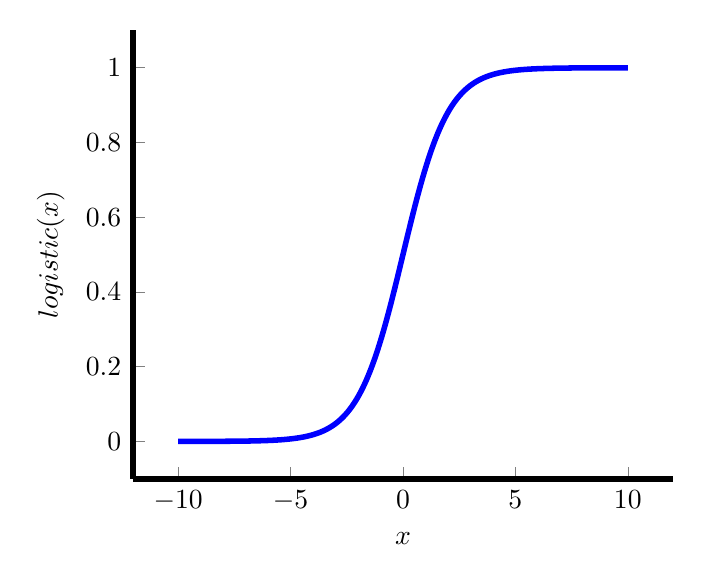
\begin{tikzpicture}
        \begin{axis}[every axis plot, line width=2pt,
                ylabel={$\text{logistic}(x)$},
                xlabel={$x$},
                domain=-10:10,samples=200,
                axis x line*=bottom, % no box around the plot, only x and y axis
                axis y line*=left % the * suppresses the arrow tips
            ]

            \addplot [blue] (x,{1/(1+exp(-x))});
        \end{axis}
    \end{tikzpicture}
\end{frame}

\subsubsection{Probit Function}
\begin{frame}{Probit Function}
    We can also opt to choose to use the \textbf{probit function}
    (usually represented by the Greek letter $\Phi$)
    which is the CDF of a normal distribution:
    $$
        \Phi (x)= \frac {1}{\sqrt {2 \pi}}\int _{-\infty }^{x}e^{-t^{2}/2}\,dt
    $$
\end{frame}

\begin{frame}{Probit Function}
    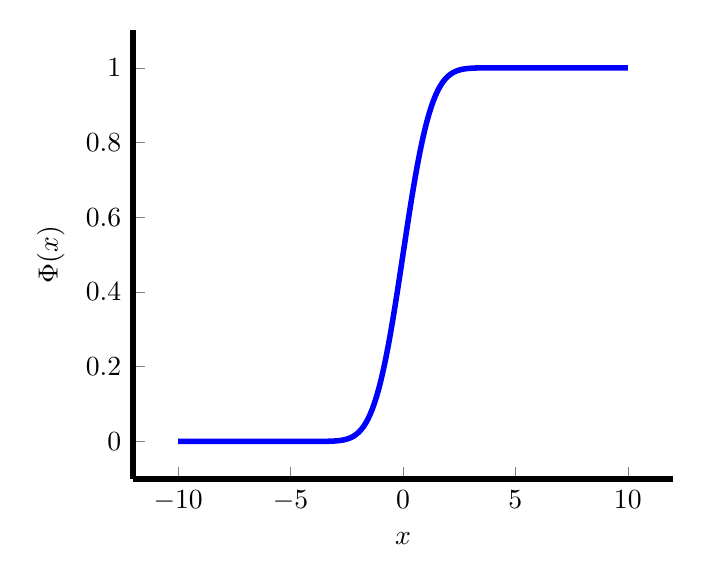
\begin{tikzpicture}
        \begin{axis}[every axis plot, line width=2pt,
                ylabel={$\Phi(x)$},
                xlabel={$x$},
                domain=-10:10,samples=200,
                axis x line*=bottom, % no box around the plot, only x and y axis
                axis y line*=left % the * suppresses the arrow tips
            ]

            \addplot [blue] {normcdf(0, 1)};
        \end{axis}
    \end{tikzpicture}
\end{frame}

\subsubsection{Logistic Function versus Probit Function}
\begin{frame}{Logistic Function versus Probit Function}
    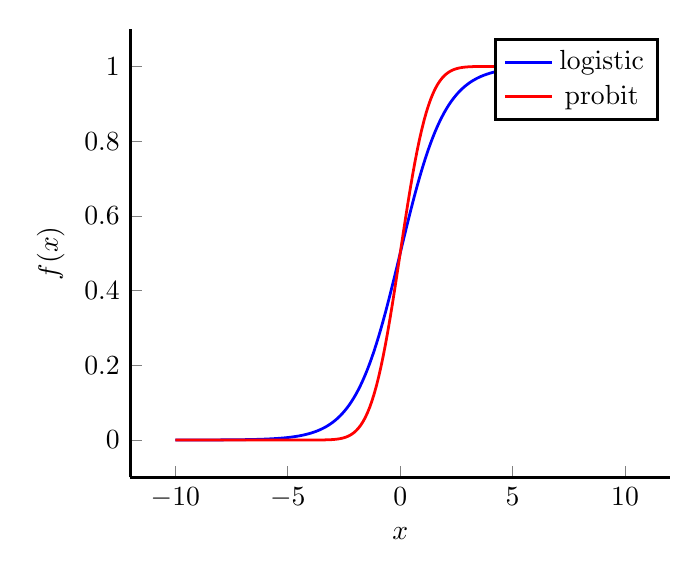
\begin{tikzpicture}
        \begin{axis}[every axis plot, line width=1pt,
                ylabel={$f(x)$},
                xlabel={$x$},
                domain=-10:10,samples=200,
                axis x line*=bottom, % no box around the plot, only x and y axis
                axis y line*=left % the * suppresses the arrow tips
            ]
            \addplot [blue] (x,{1/(1+exp(-x))});
            \addlegendentry{logistic}
            \addplot [red] {normcdf(0, 1)};
            \addlegendentry{probit}
        \end{axis}
    \end{tikzpicture}
\end{frame}

\subsection{Comparison with Linear Regression}
\begin{frame}{Comparison with Linear Regression}
    Linear regression follows the following mathematical expression:
    \small
    $$
        \text{linear} = \alpha + \beta_1 x_1 + \beta_2 x_2 + \dots + \beta_k x_k
    $$
    \begin{vfilleditems}
        \item \small $\alpha$ -- intercept.
        \item \small $\boldsymbol{\beta} = \beta_1, \beta_2, \dots, \beta_k$ -- independent variables' $x_1, x_2, \dots, x_k$ coefficients.
        \item \small $k$ -- number of independent variables.
    \end{vfilleditems}
    If you implement a small mathematical transformation,
    you'll have \textbf{logistic regression}:
    \begin{vfilleditems}
        \item \small $\hat{p} = \text{logistic}(\text{linear}) = \frac{1}{1 + e^{-\operatorname{linear}}}$ --
        probability of an observation taking value $1$.
        \item \small $\hat{y} = \begin{cases} 0 & \text { if } \hat{p} < 0.5 \\ 1 & \text { if } \hat{p} \geq 0.5 \end{cases}$ --
        $\mathbf{y}$'s predicted binary value.
    \end{vfilleditems}
\end{frame}

\subsection{Logistic Regression Specification}
\begin{frame}{Logistic Regression Specification}
    We can model logistic regression using two approaches:
    \begin{vfilleditems}
        \item \textbf{Bernoulli likelihood} --
        \textbf{binary} dependent variable \textbf{y} which results from a
        Bernoulli trial with some probability $p$
        \item \textbf{binomial likelihood} --
        \textbf{discrete and positive} dependent variable $\textbf{y}$
        which results from $k$ successes in $n$ independent Bernoulli
        trials.
    \end{vfilleditems}
\end{frame}

\subsubsection{Bernoulli Likelihood}
\begin{frame}{Bernoulli Likelihood}
    \small
    $$
        \begin{aligned}
            \mathbf{y}         & \sim \text{Bernoulli}\left( p\right)                                      \\
            p                  & = \text{logistic/probit}(\alpha +  \mathbf{X} \boldsymbol{\beta})          \\
            \alpha             & \sim \text{Normal}(\mu_\alpha, \sigma_\alpha)                             \\
            \boldsymbol{\beta} & \sim \text{Normal}(\mu_{\boldsymbol{\beta}}, \sigma_{\boldsymbol{\beta}})
        \end{aligned}
    $$
    where:
    \begin{vfilleditems}
        \item \small $\mathbf{y}$ - \textbf{dependent binary variable}.
        \item \small $p$ - probability of $\mathbf{y}$ taking value of $1$ --
        success in an independent Bernoulli trial.
        \item \small $\text{logistic/probit}$ -- logistic or probit function.
        \item \small $\alpha$ -- intercept (also called constant).
        \item \small $\boldsymbol{\beta}$ -- coefficient vector.
        \item \small $\mathbf{X}$ -- data matrix.
    \end{vfilleditems}
\end{frame}

\subsubsection{Binomial Likelihood}
\begin{frame}{Binomial Likelihood}
    \small
    $$
        \begin{aligned}
            \mathbf{y}         & \sim \text{Binomial}\left(n,  p\right)                                    \\
            p                  & = \text{logistic/probit}(\alpha +  \mathbf{X} \boldsymbol{\beta})         \\
            \alpha             & \sim \text{Normal}(\mu_\alpha, \sigma_\alpha)                             \\
            \boldsymbol{\beta} & \sim \text{Normal}(\mu_{\boldsymbol{\beta}}, \sigma_{\boldsymbol{\beta}})
        \end{aligned}
    $$
    where:
    \begin{vfilleditems}
        \item \small $\mathbf{y}$ - \textbf{discrete positive variable} -- $k$ successes of $n$ independent Bernoulli trials.
        \item \small $n$ - number of independent Bernoulli trials.
        \item \small $p$ - probability of $\mathbf{y}$ taking value of $1$ --
        success in an independent Bernoulli trial.
        \item \small $\text{logistic/probit}$ -- logistic or probit function.
        \item \small $\alpha$ -- intercept (also called constant).
        \item \small $\boldsymbol{\beta}$ -- coefficient vector.
        \item \small $\mathbf{X}$ -- data matrix.
    \end{vfilleditems}
\end{frame}
\subsection{Bayesian Logistic Regression in Pumas}
\begin{frame}{Bayesian Logistic Regression in Pumas}
    \centering
    \includegraphics[width=0.4\columnwidth]{log_reg.png}
\end{frame}

%!TEX root = slides.tex

\section{Hierarchical Models}

\subsection{Hierarchical Models - Recommended References}
\begin{frame}{Hierarchical Models - Recommended References}
	\begin{vfilleditems}
		\item \textcite{gelman2013bayesian}:
		\begin{vfilleditems}
			\item Chapter 5: Hierarchical models
			\item Chapter 15: Hierarchical linear models
		\end{vfilleditems}
		\item \textcite{mcelreath2020statistical}:
		\begin{vfilleditems}
			\item Chapter 13: Models With Memory
			\item Chapter 14: Adventures in Covariance
		\end{vfilleditems}
		\item \textcite{gelmanDataAnalysisUsing2007}
		\item Michael Betancourt's case study on \href{https://betanalpha.github.io/assets/case_studies/hierarchical_modeling.html}{Hierarchical modeling}
		\item \textcite{kruschke2015bayesian}
	\end{vfilleditems}
\end{frame}

\subsection{What are hierarchical models?}
\begin{frame}{I have many names...}
	Hierarchical models are also known for several names\footnote{
		for the whole full list
		\href{https://statmodeling.stat.columbia.edu/2019/09/18/all-the-names-for-hierarchical-and-multilevel-modeling/}{check here}.}:
	\begin{vfilleditems}
		\item Hierarchical Models
		\item Random Effects Models
		\item Mixed Effects Models
		\item Cross-Sectional Models
		\item Nested Data Models
	\end{vfilleditems}
\end{frame}

\begin{frame}{What are hierarchical models?}
	\begin{defn}[Hierarchical Model]
		Statistical model specified in multiple levels that estimates
		parameters from the posterior distribution using a Bayesian approach.
		The sub-models inside the model combines to form a hierarchical model,
		and Bayes' theorem is used to integrate it to observed data and
		account for all uncertain.
	\end{defn}
	\vfill
	Hierarchical models are mathematical descriptions that involves several parameters,
	where some parameters' estimates depend on another parameters' values.
\end{frame}

\begin{frame}{What are Hierarchical Models?\footnote{figure adapted from \href{https://betanalpha.github.io/assets/case_studies/hierarchical_modeling.html}{Michael Betancourt (CC-BY-SA-4.0)}}}
	\small
	Hyperparameter $\omega$ that parameterizes $\eta_1, \eta_2, \dots, \eta_K$,
	that are used to define the distribution of some observations
	$\mathbf{y} = y_1, y_2, \dots, y_K$
	\begin{adjustbox}{max width=1.0\textwidth}
		\begin{tikzpicture}[scale=0.275, thick]

			\pgfmathsetmacro{\r}{2}
			\pgfmathsetmacro{\dx}{0}
			\pgfmathsetmacro{\dy}{0}

			\draw[black] (-21 + \dx, -7 + \dy) rectangle (21 + \dx, 13 + \dy);

			\filldraw[fill=dark, draw=dark, line width=1.5] (-12 + \dx, 9 + \dy) circle (\r)
			node[color=white] { $y_{1}$ };

			\filldraw[fill=dark, draw=dark, line width=1.5] (-6 + \dx, 9 + \dy) circle (\r)
			node[color=white] { $\ldots$ };

			\filldraw[fill=dark, draw=dark, line width=1.5] (0 + \dx, 9 + \dy) circle (\r)
			node[color=white] { $y_{k}$ };

			\filldraw[fill=dark, draw=dark, line width=1.5] (6 + \dx, 9 + \dy) circle (\r)
			node[color=white] { $\ldots$ };

			\filldraw[fill=dark, draw=dark, line width=1.5] (12 + \dx, 9 + \dy) circle (\r)
			node[color=white] { $y_{K}$ };

			\draw[->, >=stealth, color=mid, line width=1.5] (-12 + \dx, 3 + \r + \dy) -- (-12 + \dx, 9 - \r + \dy);
			\draw[->, >=stealth, color=mid, line width=1.5] (-6 + \dx, 3 + \r + \dy) -- (-6 + \dx, 9 - \r + \dy);
			\draw[->, >=stealth, color=mid, line width=1.5] (0 + \dx, 3 + \r + \dy) -- (0 + \dx, 9 - \r + \dy);
			\draw[->, >=stealth, color=mid, line width=1.5] (6 + \dx, 3 + \r + \dy) -- (6 + \dx, 9 - \r + \dy);
			\draw[->, >=stealth, color=mid, line width=1.5] (12 + \dx, 3 + \r + \dy) -- (12 + \dx, 9 - \r + \dy);

			\filldraw[fill=black, draw=dark, line width=1.5] (-12 + \dx, 3 + \dy) circle (\r)
			node[color=white] { $\eta_{1}$ };

			\filldraw[fill=black, draw=dark, line width=1.5] (-6 + \dx, 3 + \dy) circle (\r)
			node[color=white] { $\ldots$ };

			\filldraw[fill=black, draw=dark, line width=1.5] (0 + \dx, 3 + \dy) circle (\r)
			node[color=white] { $\eta_{k}$ };

			\filldraw[fill=black, draw=dark, line width=1.5] (6 + \dx, 3 + \dy) circle (\r)
			node[color=white] { $\ldots$ };

			\filldraw[fill=black, draw=dark, line width=1.5] (12 + \dx, 3 + \dy) circle (\r)
			node[color=white] { $\eta_{K}$ };

			\draw[->, >=stealth, color=mid, line width=1.5] (0 + \dx, -3 + \r + \dy) -- (-12 + \dx, 3 - \r + \dy);
			\draw[->, >=stealth, color=mid, line width=1.5] (0 + \dx, -3 + \r + \dy) -- (-6 + \dx, 3 - \r + \dy);
			\draw[->, >=stealth, color=mid, line width=1.5] (0 + \dx, -3 + \r + \dy) -- (0 + \dx, 3 - \r + \dy);
			\draw[->, >=stealth, color=mid, line width=1.5] (0 + \dx, -3 + \r + \dy) -- (6 + \dx, 3 - \r + \dy);
			\draw[->, >=stealth, color=mid, line width=1.5] (0 + \dx, -3 + \r + \dy) -- (12 + \dx, 3 - \r + \dy);

			\filldraw[fill=black, draw=dark, line width=1.5] (0 + \dx, -3 + \dy) circle (\r)
			node[color=white] { $\omega$ };

		\end{tikzpicture}
	\end{adjustbox}
\end{frame}

\begin{frame}{What are Hierarchical Models?\footnote{figure adapted from \href{https://betanalpha.github.io/assets/case_studies/hierarchical_modeling.html}{Michael Betancourt (CC-BY-SA-4.0)}}}
	\footnotesize
	Even that the observations directly inform only a single set of parameters,
	a hierarchical model couples individual parameters,
	and provides a ``backdoor'' for information flow.
	\begin{adjustbox}{max width=1.0\textwidth}
		\begin{tikzpicture}[scale=0.3, thick]

			% Right
			\pgfmathsetmacro{\r}{2}

			\pgfmathsetmacro{\dx}{0}
			\pgfmathsetmacro{\dy}{0}

			\draw[black] (-17 + \dx, -7 + \dy) rectangle (17 + \dx, 13 + \dy);

			\fill[fill=dark, line width=1.5, opacity=0.50] (-12 + \dx, 9 + \dy) circle (\r)
			node[color=white] { $y_{1}$ };

			\fill[fill=dark, line width=1.5, opacity=0.50] (-6 + \dx, 9 + \dy) circle (\r)
			node[color=white] { $\ldots$ };

			\filldraw[fill=dark, draw=dark, line width=1.5] (0 + \dx, 9 + \dy) circle (\r)
			node[color=white] { $y_{k}$ };

			\fill[fill=dark, line width=1.5, opacity=0.50] (6 + \dx, 9 + \dy) circle (\r)
			node[color=white] { $\ldots$ };

			\fill[fill=dark, line width=1.5, opacity=0.50] (12 + \dx, 9 + \dy) circle (\r)
			node[color=white] { $y_{K}$ };

			\draw[<-, >=stealth, color=dark, line width=1.5] (0 + \dx, 3 + \r + \dy) -- (0 + \dx, 9 - \r + \dy);

			\filldraw[fill=black, draw=dark, line width=1.5] (-12 + \dx, 3 + \dy) circle (\r)
			node[color=white] { $\eta_{1}$ };

			\filldraw[fill=black, draw=dark, line width=1.5,] (-6 + \dx, 3 + \dy) circle (\r)
			node[color=white] { $\ldots$ };

			\filldraw[fill=black, draw=dark, line width=1.5] (0 + \dx, 3 + \dy) circle (\r)
			node[color=white] { $\eta_{k}$ };

			\filldraw[fill=black, draw=dark, line width=1.5] (6 + \dx, 3 + \dy) circle (\r)
			node[color=white] { $\ldots$ };

			\filldraw[fill=black, draw=dark, line width=1.5] (12 + \dx, 3 + \dy) circle (\r)
			node[color=white] { $\eta_{K}$ };

			\draw[->, >=stealth, color=dark, line width=1.5] (0 + \dx, -3 + \r + \dy) -- (-12 + \dx, 3 - \r + \dy);
			\draw[->, >=stealth, color=dark, line width=1.5] (0 + \dx, -3 + \r + \dy) -- (-6 + \dx, 3 - \r + \dy);
			\draw[<-, >=stealth, color=dark, line width=1.5] (0 + \dx, -3 + \r + \dy) -- (0 + \dx, 3 - \r + \dy);
			\draw[->, >=stealth, color=dark, line width=1.5] (0 + \dx, -3 + \r + \dy) -- (6 + \dx, 3 - \r + \dy);
			\draw[->, >=stealth, color=dark, line width=1.5] (0 + \dx, -3 + \r + \dy) -- (12 + \dx, 3 - \r + \dy);

			\filldraw[fill=black, draw=dark, line width=1.5] (0 + \dx, -3 + \dy) circle (\r)
			node[color=white] { $\omega$ };

			% Left
			\pgfmathsetmacro{\dx}{35}
			\pgfmathsetmacro{\dy}{0}

			\draw[black] (-17 + \dx, -7 + \dy) rectangle (17 + \dx, 13 + \dy);

			\filldraw[fill=dark,  draw=dark, line width=1.5] (-12 + \dx, 9 + \dy) circle (\r)
			node[color=white] { $y_{1}$ };

			\filldraw[fill=dark,  draw=dark, line width=1.5] (-6 + \dx, 9 + \dy) circle (\r)
			node[color=white] { $\ldots$ };

			\fill[fill=dark, line width=1.5, opacity=0.50] (0 + \dx, 9 + \dy) circle (\r)
			node[color=white] { $y_{k}$ };

			\filldraw[fill=dark, draw=dark, line width=1.5] (6 + \dx, 9 + \dy) circle (\r)
			node[color=white] { $\ldots$ };

			\filldraw[fill=dark, draw=dark, line width=1.5] (12 + \dx, 9 + \dy) circle (\r)
			node[color=white] { $y_{K}$ };

			\draw[<-, >=stealth, color=dark, line width=1.5] (-12 + \dx, 3 + \r + \dy) -- (-12 + \dx, 9 - \r + \dy);
			\draw[<-, >=stealth, color=dark, line width=1.5] (-6 + \dx, 3 + \r + \dy) -- (-6 + \dx, 9 - \r + \dy);
			\draw[<-, >=stealth, color=dark, line width=1.5] (6 + \dx, 3 + \r + \dy) -- (6 + \dx, 9 - \r + \dy);
			\draw[<-, >=stealth, color=dark, line width=1.5] (12 + \dx, 3 + \r + \dy) -- (12 + \dx, 9 - \r + \dy);

			\filldraw[fill=black, draw=dark, line width=1.5] (-12 + \dx, 3 + \dy) circle (\r)
			node[color=white] { $\eta_{1}$ };

			\filldraw[fill=black, draw=dark, line width=1.5,] (-6 + \dx, 3 + \dy) circle (\r)
			node[color=white] { $\ldots$ };

			\filldraw[fill=black, draw=dark, line width=1.5] (0 + \dx, 3 + \dy) circle (\r)
			node[color=white] { $\eta_{k}$ };

			\filldraw[fill=black, draw=dark, line width=1.5] (6 + \dx, 3 + \dy) circle (\r)
			node[color=white] { $\ldots$ };

			\filldraw[fill=black, draw=dark, line width=1.5] (12 + \dx, 3 + \dy) circle (\r)
			node[color=white] { $\eta_{K}$ };

			\draw[<-, >=stealth, color=dark, line width=1.5] (-\r + \dx, -3 + \dy) -- (-12 + \dx, 3 - \r + \dy);
			\draw[<-, >=stealth, color=dark, line width=1.5] ({-0.25 - \r * cos(45) + \dx}, {-3 + \r * cos(45) + \dy}) -- (-6 + \dx, 3 - \r + \dy);
			\draw[->, >=stealth, color=dark, line width=1.5] (0 + \dx, -3 + \r + \dy) -- (0 + \dx, 3 - \r + \dy);
			\draw[<-, >=stealth, color=dark, line width=1.5] ({0.25 + \r * cos(45) + \dx}, {-3 + \r * cos(45) + \dy}) -- (6 + \dx, 3 - \r + \dy);
			\draw[<-, >=stealth, color=dark, line width=1.5] (\r + \dx, -3 + \dy) -- (12 + \dx, 3 - \r + \dy);

			\filldraw[fill=black, draw=dark, line width=1.5] (0 + \dx, -3 + \dy) circle (\r)
			node[color=white] { $\omega$ };
		\end{tikzpicture}
	\end{adjustbox}

	\footnotesize
	For example, the observations from the $k$th group, $y_k$,
	informs directly the parameters that quantify the $k$th group's behavior,
	$\eta_k$.
	These parameters, however, inform directly the population-level parameters,
	$\omega$, that, in turn, informs others group-level parameters.
	In the same manner, observations that informs directly other group's parameters
	also provide indirectly information to population-level parameters,
	which then informs other group-level parameters, and so on...
\end{frame}

\subsection{When to Use Hierarchical Models?}
\begin{frame}{When to Use Hierarchical Models?}
	\textbf{Hierarchical models} are used when information is available in
	\textbf{several levels of units of observation}.
	The hierarchical structure of analysis and organization assists in the
	understanding of \textbf{multiparameter problems},
	while also performing a crucial role in the development of
	\textbf{computational strategies}.
\end{frame}

\begin{frame}{When to Use Hierarchical Models?}
	Hierarchical models are particularly appropriate for research projects
	where participant data can be organized in more than one level\footnote{
		also known as nested data.}.
	The units of analysis are generally individuals that are nested inside
	contextual/aggregate units (groups).
	\vfill
	\small
	An example is when we measure individual performance
	and we have additional information about distinct group membership such as:
	\begin{vfilleditems}
		\item \small sex
		\item \small age group
		\item \small income level
		\item \small education level
		\item \small state/province of residence
	\end{vfilleditems}
\end{frame}

\begin{frame}{When to Use Hierarchical Models?}
	Another good use case is \textbf{big data} \parencite{gelman2013bayesian}.
	\begin{vfilleditems}
		\item simple nonhierarchical models are usually inappropriate for hierarchical data:
		with few parameters,
		they generally \textit{cannot} fit large datasets accurately.
		\item whereas with many parameters, they tend to \textbf{overfit}.
		\item hierarchical models can have enough parameters to fit the data well,
		while using a population distribution to structure some dependence into the parameters,
		thereby \textbf{avoiding problems of overfitting}.
	\end{vfilleditems}
\end{frame}

\begin{frame}{When to Use Hierarchical Models?}
	Most important is \textbf{not to violate} the \textbf{exchangeability assumption}
	\parencite{definettiTheoryProbability1974}.
	\vfill
	This assumption stems from the principle that \textbf{groups are \textit{exchangeable}}.
\end{frame}

\begin{frame}{Exchangeability \parencite{definettiTheoryProbability1974}\footnote{figures adapted from \href{https://betanalpha.github.io/assets/case_studies/hierarchical_modeling.html}{Michael Betancourt (CC-BY-SA-4.0)}.}}
	\begin{adjustbox}{max width=1.0\textwidth}
		\begin{tikzpicture}[scale=0.3, thick]

			% Left
			\begin{scope}[shift={(-36, 0)}]

				\draw[white] (-17, 0) rectangle (17, 15);

				\fill[dark] (-10, 4) circle (1);
				\begin{scope}
					\clip (-10, 4) circle (1);
					\draw[color=light, line width=5, rotate=30] (-5.25, 8.25) arc[x radius=1.4, y radius=0.2, start angle=0, end angle=-180];
				\end{scope}
				\node at (-10, 10) {\includegraphics[width=2cm]{cup_up.png}};

				\fill[mid] (0, 4) circle (1);
				\begin{scope}
					\clip (0, 4) circle (1);
					\draw[color=dark, line width=2] (1.1, 4.3) arc[x radius=1.1, y radius=0.2, start angle=0, end angle=180];
					\draw[color=dark, line width=2] (1.1, 3.7) arc[x radius=1.1, y radius=0.2, start angle=0, end angle=180];
				\end{scope}
				\node at (0, 10) {\includegraphics[width=2cm]{cup_up.png}};

				\fill[dark] (+10, 4) circle (1);
				\begin{scope}
					\clip (10, 4) circle (1);
					\draw[color=mid, line width=1] (10, 3) -- (10, 5);
					\draw[color=mid, line width=1] (10.25, 5) arc[x radius=0.3, y radius=1.1, start angle=90, end angle=-90];
					\draw[color=mid, line width=1] (9.75, 5) arc[x radius=0.3, y radius=1.1, start angle=90, end angle=270];
				\end{scope}
				\node at (+10, 10) {\includegraphics[width=2cm]{cup_up.png}};

			\end{scope}

			% Right
			\begin{scope}[shift={(0, 0)}]

				\draw[white] (-17, 0) rectangle (17, 15);

				\fill[dark] (-10, 4) circle (1);
				\node at (-10, 7) {\includegraphics[width=2cm]{cup_down.png}};
				\begin{scope}[scale=0.7, shift={(-17, 3)}, rotate=-5]
					\fill[dark, rounded corners=3] (0, 0) rectangle (10, 6);
					\fill[black] (0, 0.5) rectangle (10, 3.5);
					\node[text=white, align=center, rotate=-5] at (5, 5.2) { \small \textsf{HELLO} };
					\node[text=white, align=center, rotate=-5] at (5, 4.1) { \tiny \textsf{my name is} };
					\node[text=white, align=center, rotate=0] at (5.25, 2) { \large \textsl{Group 1} };
				\end{scope}

				\fill[dark] (0, 4) circle (1);
				\node at (0, 7) {\includegraphics[width=2cm]{cup_down.png}};
				\begin{scope}[scale=0.7, shift={(-2, 3)}, rotate=10]
					\fill[dark, rounded corners=3] (0, 0) rectangle (10, 6);
					\fill[black] (0, 0.5) rectangle (10, 3.5);
					\node[text=white, align=center, rotate=10] at (5, 5.2) { \small \textsf{HELLO} };
					\node[text=white, align=center, rotate=10] at (5, 4.1) { \tiny \textsf{my name is } };
					\node[text=white, align=center, rotate=7] at (5.25, 2) { \large \textsl{Group 2} };
				\end{scope}

				\fill[dark] (+10, 4) circle (1);
				\node at (+10, 7) {\includegraphics[width=2cm]{cup_down.png}};
				\begin{scope}[scale=0.7, shift={(12, 3)}, rotate=1]
					\fill[dark, rounded corners=3] (0, 0) rectangle (10, 6);
					\fill[black] (0, 0.5) rectangle (10, 3.5);
					\node[text=white, align=center, rotate=1] at (5, 5.2) { \small \textsf{HELLO} };
					\node[text=white, align=center, rotate=1] at (5, 4.1) { \tiny \textsf{my name is } };
					\node[text=white, align=center, rotate=1] at (5.25, 2) { \large \textsl{Group 3} };
				\end{scope}
			\end{scope}
		\end{tikzpicture}
	\end{adjustbox}
\end{frame}

\begin{frame}{Exchangeability \parencite{definettiTheoryProbability1974}\footnote{figures adapted from \href{https://betanalpha.github.io/assets/case_studies/hierarchical_modeling.html}{Michael Betancourt (CC-BY-SA-4.0)}.}}
	\begin{adjustbox}{max width=1.0\textwidth}
		\begin{tikzpicture}[scale=0.3, thick]


			\draw[white] (-17, -3) rectangle (17, 15);

			\fill[dark] (-10, 4) circle (1);
			\node at (-10, 7) {\includegraphics[width=2cm]{cup_down.png}};

			% Left
			\begin{scope}[scale=0.7, shift={(-17, 3)}, rotate=-5]
				\fill[dark, rounded corners=3] (0, 0) rectangle (10, 6);
				\fill[black] (0, 0.5) rectangle (10, 3.5);
				\node[text=white, align=center, rotate=-5] at (5, 5.2) { \small \textsf{HELLO} };
				\node[text=white, align=center, rotate=-5] at (5, 4.1) { \tiny \textsf{my name is } };
				\node[text=white, align=center, rotate=0] at (5.25, 2) { \large \textsl{Group 1} };
			\end{scope}

			\fill[dark] (0, 4) circle (1);
			\node at (0, 7) {\includegraphics[width=2cm]{cup_down.png}};

			\begin{scope}[scale=0.7, shift={(-2, 3)}, rotate=10]
				\fill[dark, rounded corners=3] (0, 0) rectangle (10, 6);
				\fill[black] (0, 0.5) rectangle (10, 3.5);
				\node[text=white, align=center, rotate=10] at (5, 5.2) { \small \textsf{HELLO} };
				\node[text=white, align=center, rotate=10] at (5, 4.1) { \tiny \textsf{my name is } };
				\node[text=white, align=center, rotate=7] at (5.25, 2) { \large \textsl{Group 2} };
			\end{scope}

			\fill[dark] (+10, 4) circle (1);
			\node at (+10, 7) {\includegraphics[width=2cm]{cup_down.png}};

			\begin{scope}[scale=0.7, shift={(12, 3)}, rotate=1]
				\fill[dark, rounded corners=3] (0, 0) rectangle (10, 6);
				\fill[black] (0, 0.5) rectangle (10, 3.5);
				\node[text=white, align=center, rotate=1] at (5, 5.2) { \small \textsf{HELLO} };
				\node[text=white, align=center, rotate=1] at (5, 4.1) { \tiny \textsf{my name is } };
				\node[text=white, align=center, rotate=1] at (5.25, 2) { \large \textsl{Group 3} };
			\end{scope}

			\pgfmathsetmacro{\r}{10}
			\pgfmathsetmacro{\start}{160}
			\pgfmathsetmacro{\stop}{20}

			\draw[dark, <->, >=stealth] ({0 + \r * cos(\start)}, {8 + \r * sin(\start)})
			arc[x radius = \r, y radius = 3, start angle=\start, end angle= \stop];

			\pgfmathsetmacro{\r}{3}
			\pgfmathsetmacro{\start}{160}
			\pgfmathsetmacro{\stop}{20}

			\draw[dark, <->, >=stealth] ({-5 + \r * cos(\start)}, {10 + \r * sin(\start)})
			arc[x radius = \r, y radius = 0.75, start angle=\start, end angle= \stop];

			\draw[dark, <->, >=stealth] ({5 + \r * cos(\start)}, {10 + \r * sin(\start)})
			arc[x radius = \r, y radius = 0.75, start angle=\start, end angle= \stop];

			% Right
			\begin{scope}[shift={(36, 0)}]

				\draw[white] (-17, -3) rectangle (17, 15);

				\fill[dark] (-10, 4) circle (1);
				\node at (-10, 7) {\includegraphics[width=2cm]{cup_down.png}};

				\begin{scope}[scale=0.7, shift={(-17, 3)}, rotate=-5]
					\fill[dark, rounded corners=3] (0, 0) rectangle (10, 6);
					\fill[black] (0, 0.5) rectangle (10, 3.5);
					\node[text=white, align=center, rotate=-5] at (5, 5.2) { \small \textsf{HELLO} };
					\node[text=white, align=center, rotate=-5] at (5, 4.1) { \tiny \textsf{my name is } };
					\node[text=white, align=center, rotate=0] at (5.25, 2) { \large \textsl{Group 3} };
				\end{scope}

				\fill[dark] (0, 4) circle (1);
				\node at (0, 7) {\includegraphics[width=2cm]{cup_down.png}};

				\begin{scope}[scale=0.7, shift={(-2, 3)}, rotate=10]
					\fill[dark, rounded corners=3] (0, 0) rectangle (10, 6);
					\fill[black] (0, 0.5) rectangle (10, 3.5);
					\node[text=white, align=center, rotate=10] at (5, 5.2) { \small \textsf{HELLO} };
					\node[text=white, align=center, rotate=10] at (5, 4.1) { \tiny \textsf{my name is } };
					\node[text=white, align=center, rotate=7] at (5.25, 2) { \large \textsl{Group 1} };
				\end{scope}

				\fill[dark] (+10, 4) circle (1);
				\node at (+10, 7) {\includegraphics[width=2cm]{cup_down.png}};

				\begin{scope}[scale=0.7, shift={(12, 3)}, rotate=1]
					\fill[dark, rounded corners=3] (0, 0) rectangle (10, 6);
					\fill[black] (0, 0.5) rectangle (10, 3.5);
					\node[text=white, align=center, rotate=1] at (5, 5.2) { \small \textsf{HELLO} };
					\node[text=white, align=center, rotate=1] at (5, 4.1) { \tiny \textsf{my name is } };
					\node[text=white, align=center, rotate=1] at (5.25, 2) { \large \textsl{Group 2} };
				\end{scope}

				\draw[light, <->, >=stealth, line width=4]
				(-8, 6.5) .. controls (-7, 7.5) and (-6.5, 8.25) ..
				(-4.5, 8.5) .. controls (-2.5, 8.75) and (-1, 8.5) .. (0, 7);
				\draw[dark, <->, >=stealth, line width=2]
				(-7.85, 6.65) .. controls (-7, 7.5) and (-6.5, 8.25) ..
				(-4.5, 8.5) .. controls (-2.5, 8.75) and (-1, 8.5) .. (-0.15, 7.15);

				\draw[light, <->, >=stealth, line width=4]
				(3, 7.5) .. controls (4, 9) and (6.25, 9.75) ..
				(8.25, 9.5) .. controls (10.25, 9.25) and (11, 8.75) .. (12, 6.75);
				\draw[dark, <->, >=stealth, line width=2]
				(3.15, 7.65) .. controls (4, 9) and (6.25, 9.75) ..
				(8.25, 9.5) .. controls (10.25, 9.25) and (11, 8.75) .. (11.9, 6.9);

				\draw[light, <->, >=stealth, line width=4]
				(-8, 1.5) .. controls (-7, -1.5) and (2, -1.25) ..
				(4, -1) .. controls (6, -0.75) and (11, -0.5) .. (12, 1.5);
				\draw[dark, <->, >=stealth, line width=2]
				(-7.925, 1.25) .. controls (-7, -1.5) and (2, -1.25) ..
				(4, -1) .. controls (6, -0.75) and (11, -0.5) .. (11.9, 1.3);

			\end{scope}

		\end{tikzpicture}
	\end{adjustbox}
\end{frame}

\subsection{Hyperprior}
\begin{frame}{Hyperprior}
	In hierarchical models, we have a hyperprior,
	which is a prior's prior:
	$$
		\begin{aligned}
			\mathbf{y}        & \sim \text{Normal}(10, \boldsymbol{\eta}) \\
			\boldsymbol{\eta} & \sim \text{Normal}(0, \omega)             \\
			\omega            & \sim \text{Normal}^+(1)
		\end{aligned}
	$$
	Here $\mathbf{y}$ is a variable of interest that belongs to distinct groups.
	$\boldsymbol{\eta}$, a prior for $\mathbf{y}$,
	is a vector of group-level parameters with their own prior
	(which becomes a hyperprior) $\omega$.
\end{frame}

\subsection{Mathematical Specification of Hierarchical Models}
\begin{frame}{Mathematical Specification of Hierarchical Models}
	We have $N$ observations organized in $J$ groups with $K$ covariates.
	$$
		\begin{aligned}
			\mathbf{y}          & \sim \text{Normal}(\mathbf{X} \boldsymbol{\eta_{j}}, \sigma)                                                       \\
			\boldsymbol{\eta_j} & \sim \text{Multivariate Normal}(\mathbf{0}, \boldsymbol{\Omega})
			\quad \text{for}\quad j \in \{ 1, \dots, J \}                                                                                            \\
			\boldsymbol{\Omega} & = \operatorname{Diagonal}(\boldsymbol{\omega}) \cdot \mathbf{C} \cdot \operatorname{Diagonal}(\boldsymbol{\omega}) \\
			\boldsymbol{\omega} & \sim \text{Normal}(0, 0.4)                                                                                         \\
			\mathbf{C}          & \sim \text{LKJ}(\eta)                                                                                              \\
			\sigma              & \sim \text{Exponential}(1)
		\end{aligned}
	$$
	Each coefficient vector $\boldsymbol{\eta}_j$ represents the
	model columns $\mathbf{X}$ coefficients for every group $j \in J$.
\end{frame}

\begin{frame}{Mathematical Specification of Hierarchical Models}
	If you need to extend to more than one group,
	such as $J_1, J_2, \dots$:
	$$
		\begin{aligned}
			\mathbf{y}             & \sim \text{Normal}(\alpha + \mathbf{X} \boldsymbol{\eta_{j1}} + \mathbf{X} \boldsymbol{\eta_{j2}}, \sigma)               \\
			\boldsymbol{\eta_{j1}} & \sim \text{Multivariate Normal}(\mathbf{0}, \boldsymbol{\Omega}_1)
			\quad \text{for}\quad j_1 \in \{ 1, \dots, J_1 \}                                                                                                 \\
			\boldsymbol{\eta_{j2}} & \sim \text{Multivariate Normal}(\mathbf{0}, \boldsymbol{\Omega}_2)
			\quad \text{for}\quad j_2 \in \{ 1, \dots, J_2 \}                                                                                                 \\
			\boldsymbol{\Omega_1}  & = \operatorname{Diagonal}(\boldsymbol{\omega_1}) \cdot \mathbf{C_1} \cdot \operatorname{Diagonal}(\boldsymbol{\omega_2}) \\
			\boldsymbol{\Omega_1}  & = \operatorname{Diagonal}(\boldsymbol{\omega_1}) \cdot \mathbf{C_2} \cdot \operatorname{Diagonal}(\boldsymbol{\omega_2}) \\
			\mathbf{C_1}           & \sim \text{LKJ}(\eta_1)                                                                                                  \\
			\mathbf{C_2}           & \sim \text{LKJ}(\eta_2)                                                                                                  \\
			\sigma                 & \sim \text{Exponential}(1)
		\end{aligned}
	$$
\end{frame}

\section{Bayesian Population Pharmacokinetic Modeling}

\subsection{Recommended References}
\begin{frame}{Bayesian Population Pharmacokinetic Modeling - Recommended References}
    \begin{vfilleditems}
        \item \textcite{Gabrielsson2006PKPDbook}:
        \begin{vfilleditems}
            \item Chapter 1: General Principles
            \item Chapter 2: Pharmacokinetic Concepts
        \end{vfilleditems}
        \item \textcite{Bonate2011PKPDbook}:
        \begin{vfilleditems}
            \item Chapter 10: Bayesian Modeling regression
        \end{vfilleditems}
        \item \textcite{margossian2022torsten}
    \end{vfilleditems}
\end{frame}

\subsection{Population Pharmacokinetic Models}
\begin{frame}{Population Pharmacokinetic Models}
    Most of the Pharmacokinetic data comes from multiple subjects
    \vfill
    How do we incorporate \textbf{between-subject variability (BSV)} into our model?
    \vfill
    Answer: Mixed-Effects
\end{frame}
%!TEX root = slides.tex

\section{Bayesian Population Pharmacodynamic Modeling}

\subsection{Recommended References}
\begin{frame}{Bayesian Population Pharmacokinetic Modeling - Recommended References}
    \begin{vfilleditems}
        \item \textcite{Gabrielsson2006PKPDbook}:
        \begin{vfilleditems}
            \item Chapter 1: General Principles
            \item Chapter 3: Pharmacodynamic Concepts
        \end{vfilleditems}
        \item \textcite{Owen2014PKPDbook}:
        \begin{vfilleditems}
            \item Chapter 10: PK/PD Models
        \end{vfilleditems}
        \item \textcite{Bonate2011PKPDbook}:
        \begin{vfilleditems}
            \item Chapter 10: Bayesian Modeling regression
        \end{vfilleditems}
        \item \textcite{margossian2022torsten}
    \end{vfilleditems}
\end{frame}

\subsection{Pharmacodynamics}
\begin{frame}{Pharmacodynamics}
    \begin{defn}[Pharmacodynamics]
        \begin{quotation}
            Pharmacodynamics can be defined as the study of the time course of the
            biological effects of drugs, the relationship of the effects to drug exposure,
            and the mechanisms of drug action.
        \end{quotation}
        \vfill \vfill
        \textcite[199]{Gabrielsson2006PKPDbook}
    \end{defn}
\end{frame}

\begin{frame}{Pharmacodynamics}
    Pharmacodynamics is generally represented as \textbf{``PD'' compartments} in a model.
    \vfill
    They can be either:
    \begin{vfilleditems}
        \item \textbf{Pharmacodynamic} (PD) models with only PD compartments
        \item \textbf{Phamacokynetic-Pharmacodynamic} (PKPD) models with both PK compartments and PD compartments
    \end{vfilleditems}
\end{frame}

\subsection{Compartment Models}
\begin{frame}{PD Compartment Models}
    There are several ways to specify (and characterize) PD compartmental models.
    \vfill
    Here we'll use the following characterization for the PD compartments:
    \begin{vfilleditems}
        \item \textbf{Impact}:
        \begin{vfilleditems}
            \item Production Rate
            \item Degradation Rate
        \end{vfilleditems}
        \item \textbf{Rate}:
        \begin{vfilleditems}
            \item Stimulation
            \item Inhibition
        \end{vfilleditems}
        \item \textbf{Effect}:
        \begin{vfilleditems}
            \item Emax
            \item Linear
            \item Sigmoid
            \item $\ldots$
        \end{vfilleditems}
    \end{vfilleditems}
\end{frame}

\begin{frame}{PD Compartment Models}
    $$
        \text{Resp}^{\prime} = \text{Resp}_0 \cdot k_{\text{out}} \cdot \operatorname{Impact}(\operatorname{Rate}, \operatorname{Effect}, \text{PK compartment}) - k_{\text{out}} \cdot \text{Resp}
    $$
    \vfill
    Example with Production Rate, Stimulation, Emax and Central PK compartment:
    $$
        \text{Resp}^{\prime} = \text{Resp}_0 \cdot k_{\text{out}} \cdot \left(1 + \frac{\text{Emax} * \text{Central}}{\text{EC}_{50} + \text{Central}} \right) - k_{\text{out}} \cdot \text{Resp}
    $$
\end{frame}

\subsection{Bayesian PD Models}
\begin{frame}{How to make it Bayesian?}
    Just put \textbf{priors} in all parameters:
    $$
        \begin{aligned}
            k_{\text{out}} & \sim \text{LogNormal}(\log{\mu_{k_{\text{out}}}}, \sigma_{k_{\text{out}}}) \\
            \text{Resp}_0  & \sim \text{LogNormal}(\log{\mu_{\text{Resp}_0}}, \sigma_{\text{Resp}_0})   \\
            \ldots
        \end{aligned}
    $$
\end{frame}

\subsection{Bayesian PopPD Models}
\begin{frame}{How to make it Bayesian?}
    Just put \textbf{priors} in all parameters:
    $$
        \begin{aligned}
            \theta   & \sim \text{Normal}(0, 2.5)  \\
            \omega   & \sim \text{Normal}^+(0, 2.5)  \\
            \eta_{i} & \sim \text{Normal}(0, \omega)
        \end{aligned}
    $$
    \vfill
    where each subject $i$ has its own $\eta_i$.
\end{frame}

\begin{frame}{Example}
    \centering
    \includegraphics[width=0.3\columnwidth]{pkpd.png}
\end{frame}

% !TeX root = slides.tex

\section{Posterior Queries and Post-processing}
\subsection{Posterior Queries}
\begin{frame}{Posterior Queries}
    $$
    \begin{aligned}
        \operatorname{E}(\theta > 0 | \text{data}) \\
        \operatorname{E}(y(\theta) | \text{data})
    \end{aligned}
    $$
\end{frame}

\subsection{Visual Predictive Check}
\begin{frame}{Visual Predictive Check}
    \centering
    \includegraphics[width=0.6\textwidth]{posterior_vpc.png}
\end{frame}

\subsection{Hands-On}
\begin{frame}{Hands-On}
\end{frame}

\include{10-MCMC}
\include{11-Marginal_MCMC}
% !TeX root = slides.tex

\section{Convergence Diagnostics}

\subsection{MCMC Convergence}
\begin{frame}{Markov Chain Convergence}
    MCMC has an interesting property that it will
    \textbf{asymptotically converge to the target distribution}\footnote{
        this property is not present on neural networks.}.
    \vfill
    That means, if we have all the time in the world, it is guaranteed,
    irrelevant of the target distribution posterior geometry,
    \textbf{MCMC will give you the right answer}.
    \vfill
    However, we don't have all the time in the world
    Different MCMC algorithms, like HMC and NUTS,
    can reduce the sampling (and warmup) time necessary for convergence to the target distribution.
\end{frame}

\begin{frame}{Can We Prove Convergence?}
    \begin{vfilleditems}
        \item In the ideal scenario, the NUTS sampler converges to the true posterior and doesn't miss on any mode.
        \item Unfortunately, this is not easy to prove in general.
        \item All the convergence diagnostics are only tests for symptoms of lack of convergence.
        \item In other words if all the diagnostics look normal, then we can't prove that the sampler didn't converge.
        \item But we also can't prove that the sampler actually converged.
    \end{vfilleditems}
\end{frame}

\begin{frame}{Signs of Lack of Convergence}
    \begin{vfilleditems}
        \item Some signs of lack of convergence are:
            \begin{vfilleditems}
                \item Any of the moments (e.g. the mean or standard deviation) is changing with time. This is diagnosed using stationarity tests by comparing different parts of a single chain to each other.
                \item Any of the moments is sensitive to the initial parameter values. This is diagnosed using multiple chains by comparing their summary statistics to each other.
            \end{vfilleditems}
        \item While high auto-correlation is not strictly a sign of lack of convergence, samplers with high auto-correlation will require many more samples to get to the same ESS as another sampler with low auto-correlation. So a low auto-correlation is usually more desirable.
    \end{vfilleditems}
\end{frame}

\subsection{Diagnostic Plots}

\begin{frame}{Trace Plot}
    \begin{columns}
        \begin{column}{0.5\textwidth}
            \centering
            \includegraphics[width=1\textwidth]{trace_1.png}
        \end{column}
        \begin{column}{0.5\textwidth}
            The trace plot of a parameter shows the value of the parameter in each iteration of the MCMC algorithm.
        \end{column}
    \end{columns}
\end{frame}

\begin{frame}{Trace Plot}
    \begin{columns}
        \begin{column}{0.5\textwidth}
            \centering
            \includegraphics[width=1\textwidth]{trace_1.png}
        \end{column}
        \begin{column}{0.5\textwidth}
            A good trace plot is one that:
            \vfill
            \begin{vfilleditems}
                \item Is noisy, not an increasing or decreasing line for example.
                \item Has a fixed mean.
                \item Has a fixed variance.
                \item Shows all chains overlapping with each other, aka chain mixing.
            \end{vfilleditems}
            \vfill
            This is an example of somewhat well mixed chains that don't indicate non-convergence.
        \end{column}
    \end{columns}
\end{frame}

\begin{frame}{Cumulative Mean Plot}
    \begin{columns}
        \begin{column}{0.5\textwidth}
            \centering
            \includegraphics[width=1\textwidth]{cummean_1.png}
        \end{column}
        \begin{column}{0.5\textwidth}
            The cumulative mean plot of a parameter shows the mean of the parameter value in each MCMC chain up to a certain iteration.
        \end{column}
    \end{columns}
\end{frame}

\begin{frame}{Cumulative Mean Plot}
    \begin{columns}
        \begin{column}{0.5\textwidth}
            \centering
            \includegraphics[width=1\textwidth]{cummean_1.png}
        \end{column}
        \begin{column}{0.5\textwidth}
            An MCMC chain converging to a stationary posterior distribution should have the cumulative mean of each parameter converge to a fixed value.
        \end{column}
    \end{columns}
\end{frame}

\begin{frame}{Cumulative Mean Plot}
    \begin{columns}
        \begin{column}{0.5\textwidth}
            \centering
            \includegraphics[width=1\textwidth]{cummean_1.png}
        \end{column}
        \begin{column}{0.5\textwidth}
            All the chains should be converging to the same mean for a given parameter, the posterior mean.
        \end{column}
    \end{columns}
\end{frame}

\begin{frame}{Density Plot}
    \begin{columns}
        \begin{column}{0.5\textwidth}
            \centering
            \includegraphics[width=1\textwidth]{density_1.png}
        \end{column}
        \begin{column}{0.5\textwidth}
            \begin{vfilleditems}
                \item The density plot of a parameter shows a smoothed version of the histogram of the parameter values, giving an approximate probability density function for the marginal posterior of the parameter considered.
                \item This helps us visualize the shape of the marginal posterior of each parameter.
            \end{vfilleditems}
        \end{column}
    \end{columns}
\end{frame}

\begin{frame}{Auto-correlation Plot}
    \begin{columns}
        \begin{column}{0.5\textwidth}
            \centering
            \includegraphics[width=1\textwidth]{corplot_1.png}
        \end{column}
        \begin{column}{0.5\textwidth}
            \begin{vfilleditems}
                \item MCMC chains are prone to auto-correlation between the samples because each sample in the chain is a function of the previous sample.
                \item The auto-correlation plot shows the correlation between every sample with index $s$ and the corresponding sample with index $s + \text{lag}$ for all $s \in 1:N-\text{lag}$ where $N$ is the total number of samples.
            \end{vfilleditems}
        \end{column}
    \end{columns}
\end{frame}

\begin{frame}{Auto-correlation Plot}
    \begin{columns}
        \begin{column}{0.5\textwidth}
            \centering
            \includegraphics[width=1\textwidth]{corplot_1.png}
        \end{column}
        \begin{column}{0.5\textwidth}
            \begin{vfilleditems}
                \item For each value of $\text{lag}$, we can compute a correlation measure between the samples and their $\text{lag}$-steps-ahead counterparts.
                \item The correlation is usually a value between 0 and 1 but can sometimes be between -1 and 0 as well.
            \end{vfilleditems}
        \end{column}
    \end{columns}
\end{frame}

\begin{frame}{Auto-correlation Plot}
    \begin{columns}
        \begin{column}{0.5\textwidth}
            \centering
            \includegraphics[width=1\textwidth]{corplot_1.png}
        \end{column}
        \begin{column}{0.5\textwidth}
            \begin{vfilleditems}
                \item The auto-correlation plot shows the $\text{lag}$ on the x-axis and the correlation value on the y-axis.
                \item For well behaving MCMC chains when $\text{lag}$ increases, the corresponding correlation gets closer to 0.
            \end{vfilleditems}
        \end{column}
    \end{columns}
\end{frame}

\begin{frame}{Auto-correlation Plot}
    \begin{columns}
        \begin{column}{0.5\textwidth}
            \centering
            \includegraphics[width=1\textwidth]{corplot_1.png}
        \end{column}
        \begin{column}{0.5\textwidth}
            \begin{vfilleditems}
                \item This means that there is less and less correlation between any 2 samples further away from each other.
                \item The value of $\text{lag}$ where the correlation becomes close to 0 can be used to guide the thinning of the MCMC samples to extract mostly independent samples from the auto-correlated samples.
            \end{vfilleditems}
        \end{column}
    \end{columns}
\end{frame}

\begin{frame}{Ridge Line Plot}
    \begin{columns}
        \begin{column}{0.5\textwidth}
            \centering
            \includegraphics[width=1\textwidth]{ridge_1.png}
        \end{column}
        \begin{column}{0.5\textwidth}
            The ridge line plot shows similar information as the density plot in addition to the credible interval and quantile information.
        \end{column}
    \end{columns}
\end{frame}

\begin{frame}{Corner Plot}
    \centering
    \includegraphics[width=0.6\textwidth]{corner_1.png}
\end{frame}

\subsection{Other Diagnostics}
\begin{frame}{Convergence Metrics}
    There are a few metrics and diagnostics usually used to assess and diagnose the Markov chains:
    \begin{vfilleditems}
        \item \textbf{Effective Sample Size} (ESS):
        an approximation of the ``number of independent samples'' generated by a Markov chain.
        \item $\widehat{R}$ (\textbf{Rhat}):
        potential scale reduction factor,
        a metric to measure if the Markov chain have mixed,
        and, potentially, converged.
    \end{vfilleditems}
\end{frame}

\begin{frame}{Effective Sample Size \parencite{gelman2013bayesian}}
    $$\widehat{n}_{\text{eff}} = \frac{mn}{1 + \sum_{t=1}^T \widehat{\rho}_t}$$
    Where:
    \begin{vfilleditems}
        \item $m$: number of Markov chains.
        \item $n$: total samples per Markov chain (discarding warmup).
        \item $\widehat{\rho}_t$: an autocorrelation estimate.
    \end{vfilleditems}
\end{frame}

\begin{frame}{Rhat \parencite{gelman2013bayesian}}
    $$\widehat{R} = \sqrt{\frac{\widehat{\text{var}}^+(\psi \mid y)}{W}}$$
    where $\widehat{\text{var}}^+(\psi \mid y)$ is the Markov chains' sample variance
    for a certain parameter $\psi$.
    We calculate it by using a weighted sum of the within-chain $W$
    and between-chain $B$ variances:
    $$\widehat{\text{var}}^+(\psi \mid y) = \frac{n-1}{n} W + \frac{1}{n} B$$
    \vfill
    Intuitively, the value is $1.0$ if all chains are totally convergent.
    As a heuristic, if $\widehat{R} > 1.1$,
    you need to worry because probably the chains have not converged adequate.
\end{frame}

% % plots taken from script:
% % slides/images/bad_chains_traceplot.tex
% \begin{frame}{Traceplot -- Convergent Markov Chains}
%     \begin{figure}
%         \centering
%         \resizebox{.4\linewidth}{!}{\input{images/good_chains_traceplot.tex}}
%         \caption{A convergent Markov chains traceplot}
%     \end{figure}
% \end{frame}

% \begin{frame}{Traceplot -- Divergent Markov Chains}
%     \begin{figure}
%         \centering
%         \resizebox{.4\linewidth}{!}{\input{images/bad_chains_traceplot.tex}}
%         \caption{A divergent Markov chains traceplot}
%     \end{figure}
% \end{frame}

% \subsubsection{What To Do If the Markov Chains Do Not Converge?}
% \begin{frame}[fragile]{\texttt{Stan}'s Warning Messages\footnote{also see \href{https://mc-stan.org/misc/warnings.html}{\texttt{Stan}'s \textcolor{red}{warnings} guide}.}}
%     \begin{lstlisting}[basicstyle=\footnotesize\color{red}]
% Warning messages:
% 1: There were 275 divergent transitions after warmup. See
% http://mc-stan.org/misc/warnings.html#divergent-transitions-after-warmup
% to find out why this is a problem and how to eliminate them.
% 2: Examine the pairs() plot to diagnose sampling problems

% 3: The largest R-hat is 1.12, indicating chains have not mixed.
% Running the chains for more iterations may help. See
% http://mc-stan.org/misc/warnings.html#r-hat
% 4: Bulk Effective Samples Size (ESS) is too low, indicating posterior
% means and medians may be unreliable.
% Running the chains for more iterations may help. See
% http://mc-stan.org/misc/warnings.html#bulk-ess
% 5: Tail Effective Samples Size (ESS) is too low, indicating posterior
% variances and tail quantiles may be unreliable.
% Running the chains for more iterations may help. See
% http://mc-stan.org/misc/warnings.html#tail-ess
%   \end{lstlisting}
% \end{frame}
% % https://mc-stan.org/misc/warnings.html

% \begin{frame}[fragile]{\texttt{Turing.jl}'s Warning Messages}
%     \textbf{\texttt{Turing.jl} does not give warning messages!}
%     But you can check divergent transitions with $\texttt{summarize(chn; sections=[:internals])}$:
%     \vfill
%     %@model function funnel_cp()
%     %    y ~ Normal(0, 3)
%     %    x ~ Normal(0, exp(y/2))
%     % end
%     %chn = sample(funnel_cp(), NUTS(1_000, 0.8), MCMCThreads(), 1_000, 4)
%     \begin{lstlisting}[basicstyle=\footnotesize]
% Summary Statistics
%       parameters     mean      std  naive_se     mcse      ess     rhat  ess_per_sec
%           Symbol  Float64  Float64   Float64  Float64  Float64  Float64  Float64

%               lp  -3.9649   1.7887   0.0200   0.1062  179.1235  1.0224   6.4133
%          n_steps   9.1275  11.1065   0.1242   0.7899   38.3507  1.3012   1.3731
%  acceptance_rate   0.5944   0.4219   0.0047   0.0322   40.5016  1.2173   1.4501
%       tree_depth   2.2444   1.3428   0.0150   0.1049   32.8514  1.3544   1.1762
%  numerical_error   0.1975   0.3981   0.0045   0.0273   59.8853  1.1117   2.1441
%   \end{lstlisting}
% \end{frame}

\begin{frame}{Geweke Diagnostic}
    \begin{vfilleditems}
        \item The Geweke diagnostic compares the sample means of two disjoint sub-chains $X_1$ and $X_2$ of the entire chain.
        \item It uses a difference of means hypothesis test where the null and alternative hypotheses are:
            \begin{vfilleditems}
                \item $H_0: \mu_1 = \mu_2$
                \item $H_1: \mu_1 \neq \mu_2$
            \end{vfilleditems}
        where $\mu_1$ and $\mu_2$ are the means of $X_1$ and $X_2$ respectively.
    \end{vfilleditems}
\end{frame}

\begin{frame}{Geweke Diagnostic}
    \begin{vfilleditems}
        \item The first sub-chain $X_1$ is taken as the first $(\text{first} \times 100)\%$ of the samples in the chain. The second sub-chain $X_2$ is taken as the last $(\text{last} \times 100)\%$ of the samples in the chain.
        \item The test statistic used is: $z_0 = (\bar{x}_1 - \bar{x}_2) / \sqrt{s_1^2 + s_2^2}$ where $\bar{x}_1$ and $\bar{x}_2$ are the sample means of $X_1$ and $X_2$ respectively, and $s_1$ and $s_2$ are the Markov Chain standard error (MCSE) estimates of $X_1$ and $X_2$ respectively.
        \item Auto-correlation is assumed within the samples of each individual sub-chain, but the samples in $X_1$ are assumed to be independent of the samples in $X_2$.
    \end{vfilleditems}
\end{frame}

\begin{frame}{Geweke Diagnostic}
    \begin{vfilleditems}
        \item The p-value output is an estimate of $P(|z| > |z_0|)$, where $z$ is a standard normally distributed random variable.
        \item Low p-values indicate one of the following:
            \begin{vfilleditems}
                \item The first and last parts of the chain are sampled from distributions with different means, i.e. non-convergence,
                \item The need to discard some initial samples as burn-in, or
                \item The need to run the sampling for longer due to lack of samples or high auto-correlation.
            \end{vfilleditems}
        \item High p-values (desirable) indicate the inability to conclude that the means of the first and last parts of the chain are different with statistical significance.
    \end{vfilleditems}
\end{frame}

\begin{frame}{Geweke Diagnostic}
    \begin{vfilleditems}
        \item However, this alone does not guarantee convergence to a fixed posterior distribution because:
            \begin{vfilleditems}
                \item Either the standard deviations or higher moments of $X_1$ and $X_2$ may be different, or
                \item The independence assumption between $X_1$ and $X_2$ may not be satisfied when high auto-correlation exists.
            \end{vfilleditems}
    \end{vfilleditems}
\end{frame}

\begin{frame}{Heidelberger and Welch Diagnostic}
    The Heidelberger diagnostic attempts to:
        \begin{enumerate}
            \item Identify a cutoff point for the initial transient phase for each parameter, after which the samples can be assumed to come from a steady-state posterior distribution. Can be treated as burn-in.
            \item Estimate the relative confidence interval for the mean of the steady-state posterior distribution of each parameter, assuming such steady-state distribution exists in the samples. A large confidence interval implies either the lack of convergence to a stationary distribution or lack of samples.
            \item Quantify the extent to which the distribution of the samples is stationary using a hypothesis test. The returned p-value can be considered a measure of mean stationarity. A p-value lower than $\alpha$ (e.g. $\alpha = 0.05$) implies lack of stationarity of the mean.
        \end{enumerate}
\end{frame}

\begin{frame}{Heidelberger and Welch Diagnostic}
    The Heidelberger diagnostic only tests for the mean of the distribution. Therefore, it can only be used to detect lack of convergence and not to prove convergence. In other words, even if all the numbers seem normal, one cannot conclude that the chain converged to a stationary distribution or that it converged to the true posterior.
\end{frame}

% \begin{frame}{Raftery and Lewis Diagnostic}
%     \begin{vfilleditems}
%         \item This diagnostic is used to determine the number of iterations required to estimate a specified quantile $q$ within a desired degree of accuracy.
%         \item The diagnostic is designed to determine the number of autocorrelated samples required to estimate a specified quantile $\theta_q$, such that $\Pr(\theta \le \theta_q) = q$, within a desired degree of accuracy.
%         \item In particular, if $\hat{\theta}_q$ is the estimand and $\Pr(\theta \le \hat{\theta}_q) = \hat{P}_q$ the estimated cumulative probability, then accuracy is specified in terms of $r$ and $s$, where $\Pr(q - r < \hat{P}_q < q + r) = s$. Sample sizes estimated by the diagnostic tend to be conservative (too large).
%     \end{vfilleditems}
% \end{frame}

\subsection{What To Do If the Markov Chains Do Not Converge?}
% \begin{frame}{What To Do If the Markov Chains Do Not Converge?}
%     \textbf{First}: before making any fine adjustments in the number of Markov chains
%     or the number of iterations per chain, etc.
%     Acknowledge that both \texttt{Stan}'s and \texttt{Turing.jl}'s NUTS sampler is
%     \textbf{very efficient and effective in exploring the
%         most crazy and diverse target posterior densities}.
%     \vfill
%     And the standard settings, \textbf{2,000 iterations and 4 chains},
%     works perfectly for 99\% of the time.
% \end{frame}

\begin{frame}{What To Do If the Markov Chains Do Not Converge?}
    \vfill
    \begin{quotation}
        When you have computational problems,
        often there’s a problem with your model.
    \end{quotation}
    \vfill \vfill
    \textcite{gelmanFolkTheoremStatistical2008} (Folk Theorem)
\end{frame}

% \begin{frame}{What To Do If the Markov Chains Do Not Converge?}
%     If you are experiencing convergence issues,
%     \textbf{and you've discarded that something is wrong with you model},
%     here is a few steps to try\footnote{
%         besides that,
%         maybe should be worth to do a QR decomposition in the data matrix $\mathbf{X}$,
%         thus having an orthogonal basis (non-correlated) for the sampler to explore.
%         This makes the target distribution's geometry much more friendlier,
%         in the topological/geometrical sense,
%         for the MCMC sampler explore.
%         Check the \hyperlink{appendixqr}{backup slides}.}.
%     Here listed in increasing complexity:
%     \begin{vfilleditems}
%         \item[1.] \textbf{Increase the number of iterations and chains}:
%         try first increasing the number of iterations,
%         then try increasing the number of chains.
%         (remember the default is 2,000 iterations and 4 chains).
%     \end{vfilleditems}
% \end{frame}

% \begin{frame}{What To Do If the Markov Chains Do Not Converge?}
%     \begin{vfilleditems}
%         \item[2.] \textbf{Change the HMC's warmup adaptation routine}:
%         make the HMC sampler to be more conservative in the proposals.
%         This can be changed by increasing the hyperparameter
%         \textbf{target acceptance rate of Metropolis proposals}\footnote{
%             \texttt{Stan}'s default is \texttt{0.8} and
%             \texttt{Turing.jl}'s default is \texttt{0.65}.}.
%         The maximum value is $1.0$ (not recommended).
%         Então qualquer valor entre $0.8$ e $1.0$ o torna mais conservador.
%         \item[3.] \textbf{Model reparameterization}:
%         there are two approaches.
%         Centered parameterization (CP) and non-centered parameterization (NCP).
%     \end{vfilleditems}
% \end{frame}

% \begin{frame}{What To Do If the Markov Chains Do Not Converge?}
%     \begin{vfilleditems}
%         \item[4.] \textbf{Collect more data}:
%         sometimes the model is too complex and we need a higher sample size for stable estimates.
%         \item[5.] \textbf{Rethink the model}:
%         convergence issues with an adequate sample size might be due to
%         incompatibility between priors and likelihood function(s).
%         In this case you need to rethink the whole data generating process
%         underlying the model, in which the model assumptions stems from.
%     \end{vfilleditems}
% \end{frame}

\begin{frame}{What To Do If the Markov Chains Do Not Converge?}
    \begin{vfilleditems}
        \item Dynamics-based models with complicated stiff differential equations often suffer from sensitivity to parameter values in 2 ways:
            \begin{vfilleditems}
                \item First, small changes in the parameter values may lead to extremely different dynamics and wrong predictions thus leading to rejections.
                \item And second, changes in the parameter values may make the differential equation highly stiff thus slowing down convergence or even causing divergence of the solver.
            \end{vfilleditems}
        \item In other words, MCMC for some complicated models can often run slow and fail to give good ESS values at the end.
        \item In such cases, NUTS may not always be computationally feasible.
        \item But you can try any of the following remedies and workarounds to poke at the model.
    \end{vfilleditems}
\end{frame}

\begin{frame}{What To Do If the Markov Chains Do Not Converge?}
    \begin{vfilleditems}
        \item Lower the target acceptance ratio. This may alleviate the need for a small step size and a full tree exploration.
        \item Re-parameterize your model to have less parameter dependence.
        \item Fix some parameter values to known good values, e.g. values obtained by maximum-a-posteriori (MAP) optimization.
        \item Initialize the sampling from good parameter values.
        \item Use a stronger prior around suspected good parameter values.
        \item Simplify your model, e.g. using simpler dynamics.
        \item Try the marginal MCMC algorithm \lstinline{MarginalMCMC} instead of the full joint MCMC algorithm \lstinline{BayesMCMC}.
    \end{vfilleditems}
\end{frame}

\begin{frame}{What To Do If the Markov Chains Do Not Converge?}
    \begin{vfilleditems}
        \item If you find the sampler regularly hitting the maximum tree depth of 10 in the initial exploration phase, it might make sense to decrease that initially to have quicker iterations when in the exploration phase of the study.
        \item This is effectively limiting the level of exploration in the sampling so it might make sense to use good initial values when doing this.
        \item However in the final phase of the study, it is best to make sure that the maximum tree depth is not reached by the sampler (increasing it if necessary).
        \item This might also slow down your sampling significantly so there can be a tradeoff here.
        \item It's also best to ensure that the sampler converges to the posterior when starting from multiple different random initial points using different chains.
    \end{vfilleditems}
\end{frame}

\subsection{Is Convergence Important?}

\begin{frame}{Is Convergence Important?}
    \begin{vfilleditems}
        \item Since we can't prove that the sampler explored the full posterior in general, is exploring the full posterior always absolutely necessary?
        \item That depends on what you want to do. If you are trying to answer questions about the parameters, e.g. estimating the probability that an effect is greater than or less than 0 for a go/no-go decision, then you need your sampler to sample from the true posterior.
        \item Of course, we cannot prove this in general anyways but you should generally follow all the best practices and you should not ignore signs of lack of convergence.
    \end{vfilleditems}
\end{frame}

\begin{frame}{Is Convergence Important?}
    \begin{vfilleditems}
        \item Some bad signs to watch out for if you want to sample from the true posterior are:
            \begin{vfilleditems}
                \item Non-stationarity of the samples' distribution
                \item Dependence of the samples' distribution on the initial parameters after the adaptation steps
                \item High auto-correlation in the samples after the adaptation steps
                \item Too many rejections and ODE solver divergences
                \item Low ESS values relative to the number of samples 
                \item Extremely small step sizes and hitting the maximum tree depth often
            \end{vfilleditems}
    \end{vfilleditems}
\end{frame}
\begin{frame}{Is Convergence Important?}
    \begin{vfilleditems}
        \item On the other hand, if your goal is not to answer questions about the parameters but only to make predictions using the posterior predictive distribution as an ensemble of predictions, then sampling from the true posterior may not be strictly necessary in this case.
        \item If the posterior predictive distribution gives enough accuracy and uncertainty in the predictions to reflect the uncertainty in the unseen data, then that may suffice and we can live with some imperfections in the sampling.
    \end{vfilleditems}
\end{frame}

\begin{frame}{Is Convergence Important?}
    \begin{vfilleditems}
        \item Some imperfections in the sampling include:
            \begin{vfilleditems}
                \item Having to initialize the sampler from a mode to get the sampler to work
                \item Using a low maximum tree depth and allowing the maximum to be reached
                \item Using a high target acceptance ratio to decrease exploration and sample around a mode
                \item High auto-correlation in the samples even after the adaptation steps and low relative ESS
                \item Using a few adaptation steps `nadapts`
            \end{vfilleditems}
    \end{vfilleditems}
\end{frame}

\begin{frame}{Is Convergence Important?}
    \begin{vfilleditems}
        \item If doing any or all of the above resulted in fast sampling that gives a good enough posterior predictive distribution but potentially bad posterior exploration and if predictions are what you care the most about then perhaps you don't need to sample from the true posterior in your use case.
        \item Such an imperfect solution is often satisfactory in the context of Bayesian neural networks for example where parameters are generally meaningless and we only care about predictions.
        \item Of course, we don't advocate for doing this in general since this goes against the best practices of MCMC but it's an option you have.
    \end{vfilleditems}
\end{frame}

\include{13-Model_Comparison_and_Cross-Validation}
\include{14-Software-Comparison}
\label{lastslide}

%--- References ----------------------------------------------------------%
\begingroup
\renewcommand{\insertframenumber}{}
\renewcommand{\pageword}{}
\begin{frame}[allowframebreaks, noframenumbering]{References}
	\printbibliography
\end{frame}

%--- Appendix ----------------------------------------------------------%
\appendix % do not count the following slides for the total number
\section*{Backup Slides}
\begin{frame}[noframenumbering]
	\centering
	\vfill
	{\fontsize{40}{50}\selectfont Backup Slides}
	\vfill
\end{frame}

%--- Backup Files ----------------------------------------------------------%
\include{backup-Statistical_Distributions}
\section*{How to Interpret Logistic Regression Coefficients}
\begin{frame}[noframenumbering]{How to Interpret Logistic Regression Coefficients}
    If we revisit logistic transformation mathematical expression,
    we see that, in order to interpret coefficients $\boldsymbol{\beta}$,
    we need to perform a transformation.
    \vfill
    Specifically, we need to undo the logistic transformation.
    We are looking for its inverse function.
\end{frame}

\subsection*{Probability versus Odds}
\begin{frame}[noframenumbering]{Probability versus Odds}
    \small
    But before that, we need to discern between
    \textbf{probability and odds}\footnote{mathematically speaking.}.
    \begin{vfilleditems}
        \item \small \textbf{Probability}: a real number between $0$ and $1$
        that represents the certainty that an event will occur,
        either by long-term frequencies (frequentist approach) or
        degrees of belief (Bayesian approach).
        \item \small \textbf{Odds}: a positive real number ($\mathbb{R}^+$)
        that also measures the certainty of an event happening.
        However this measure is not expressed as a probability
        (between $0$ and $1$),
        but as the \textbf{ratio between the number of results that
            generate our desired event and the number of results that
            \textit{do not} generate our desired event}:
        $$
            \text{odds} = \frac{p}{1-p}
        $$
        where $p$ is the probability.
    \end{vfilleditems}
\end{frame}

\begin{frame}[noframenumbering]{Probability versus Odds}
    $$
        \text{odds} = \frac{p}{1-p}
    $$
    where $p$ is the probability.
    \vfill
    \begin{vfilleditems}
        \item Odds with a value of $1$ is a neutral odds,
        similar to a fair coin: $p = \frac{1}{2}$
        \item Odds below $1$ decrease the probability of seeing a certain event.
        \item Odds over $1$ increase the probability of seeing a certain event.
    \end{vfilleditems}
\end{frame}

\subsection*{Logodds}
\begin{frame}[noframenumbering]{Logodds}
    If you revisit the logistic function, you'll se that the intercept $\alpha$
    and coefficients $\boldsymbol{\beta}$ are literally the \textbf{log of the odds}
    (logodds):
    $$
        \begin{aligned}
            p                  & = \text{logistic}(\alpha +  \mathbf{X} \boldsymbol{\beta} )                 \\
            p                  & = \text{logistic}(\alpha) + \text{logistic}( \mathbf{X} \boldsymbol{\beta}) \\
            p                  & = \frac{1}{1 + e^{(-\boldsymbol{\beta})}}                                   \\
            \boldsymbol{\beta} & = \log(\text{odds})
        \end{aligned}
    $$
\end{frame}

\begin{frame}[noframenumbering]{Logodds}
    Hence, the coefficients of a logistic regression are expressed in logodds,
    in which $0$ is the neutral element,
    and any number above or below it increases or decreases, respectively,
    the changes of obtaining a ``success'' in $\mathbf{y}$.
    To have a more intuitive interpretation (similar to the betting houses),
    we need to \textbf{convert the logodds into chances} by undoing the $\log$ function.
    We need to perform an \textbf{exponentiation} of $\alpha$ and $\boldsymbol{\beta}$
    values:
    $$
        \begin{aligned}
            \text{odds}(\alpha)               & = e^\alpha               \\
            \text{odds}({\boldsymbol{\beta}}) & = e^{\boldsymbol{\beta}}
        \end{aligned}
    $$
\end{frame}
% !TeX root = slides.tex

\section*{Miscellanea}
\subsection*{Normal Distribution Derivation}
\begin{frame}[plain, noframenumbering, label=appendixnormal]{How the Normal
        distribution arose\footnote{Origins can be traced back to
            Abraham de Moivre in 1738.
            A better explanation can be found by
            \href{http://www.stat.yale.edu/~pollard/Courses/241.fall2014/notes2014/Bin.Normal.pdf}{clicking here}.}}
    $$
        \begin{aligned}
            \text{Binomial}(n, k)                            & = \binom{n}{k} p^k (1-p)^{n-k}                                                \\
            n!                                               & \approx \sqrt{2 \pi n} \left(\frac{n}{e}\right)^n         & \text{(Stirling)} \\
            \lim_{n \to \infty} \binom{n}{k} p^k (1-p)^{n-k} & = \frac{1}{\sqrt{2 \pi npq}} e^{-\frac{(k - np)^2}{2npq}}
        \end{aligned}
    $$
    We know that in the binomial: $\mathrm{E} = np$ and $\mathrm{Var} = npq$; hence replacing $\mathrm{E}$ by $\mu$ and $\mathrm{Var}$ by $\sigma^2$:
    $$\lim_{n \to \infty} \binom{n}{k} p^k (1-p)^{n-k} = \frac{1}{\sigma \sqrt{2 \pi}} e^{-\frac{(k - \mu)^2}{\sigma^2}}$$
\end{frame}
\endgroup
